\chapter{Equivalence and Machine Minimization}
\label{chapter:equivAndMinimization}

\section{Introduction}
\label{labelIntroduction}

In the preceding chapters it was emphasized that the state of a finite-state machine need not be observable or even physical quantitites, and that their only function is to assist in the formulation of the input-output relationships of the machine. Consequently, any state set which fulfills this function is a satisfactory set, regardless of whether the state convey any intuitive meaning or not. This freedom inherent in the choice of a state set is quite advantageous, since it permits the replacement of one set with another set which may be considered more convenient for various purposes. More specifically, it permits one to carry out operations aiming at producing a state set which is ``optimal'' or ``minimal'' in one sense or another. In all these considerations the concept of ``equivalence'' plays a major role. As will become apparent in this and later chapters, this concept not only paves the way for more precise and more concise formulation of finite-state machines, but sheds new light on the entire problem of machine analysis (as well as synthesis).

\section{State Equivalence}
\label{sectionStateEquivalence}

In what follows, the notation $ M |\sigma $ will be used as an abbreviation for the phrase ``machine M in state $\sigma$''.

\definition \label{labelEquivalence}  State $ \sigma_i $ of machine $M_1$ and state $\sigma_j$ of machine $M_2$ are said to be \emph{equivalent}, if $M_1|\sigma_i$ and $M_2|\sigma_j$, when excited by any input sequence, yield identical output sequences. If $\sigma_i$ and $\sigma_j$ are not equivalent, they are said to be \emph{distinguishable}. $M_1$ and $M_2$ may refer to the same machine.

    Thus, $\sigma_i$ and $\sigma_j$ are equivalent if and only if there is no way of distinguishing, by observing the external terminals, between machine $M_1$ at the initial state $\sigma_i$ and Machine $M_2$ at the initial state $\sigma_j$. $\sigma_i$ and $\sigma_j$ are distinguishable if and only if there is at least one input sequence which, when applied to both $M_1|\sigma_i$ and $M_2|\sigma_j$, yields different output sequences.

    Equivalence between $\sigma_i$ and $\sigma_j$ is indicated by $\sigma_i = \sigma_j$, and distinguishability between $\sigma_i$ and $\sigma_j$ is indicated by  $\sigma_i \neq \sigma_j$. From definition \ref{labelEquivalence} it can be readily verified that state equivalence obeys the reflexive law ( $\sigma_i = \sigma_j$ ), the symmetric law ( if $\sigma_i = \sigma_j$, then $\sigma_j = \sigma_i$), and the transitive law  ( if $\sigma_i = \sigma_j$ and  $\sigma_j = \sigma_k$, then $\sigma_i = \sigma_k$). Consequently, state equivalence can be treated as an ordinary equivalence relation and applied directly to sets of states of any size. State distinguishability, on the other hand, does not obey the reflexive and transitive laws and, hence, can be applied only to pairs of states.

    In some cases equivalence or distinguishability of a pair of states belonging to the same machine can be estabilished by insoection of the transition table of this machine. Some of these cases are described by means of the following three lemmas. 

    %TODO: introduzir a subtable z_v

    \lemma \label{labelSimplyDistinct} Let $\sigma_i$ and $\sigma_j$ be states of machine M. If rows $\sigma_i$ and $\sigma_j$ in the $ z_v $ subtable of M are distinct, then $ \sigma_i \neq \sigma_j $.

    \emph{Proof}. There must be at least one input symbol which, when applied to $M|\sigma_i$ and $M|\sigma_j$, yields distinct output symbols. By definition \ref{labelEquivalence}, then $\sigma_i \neq \sigma_j$.


    \lemma \label{labelSimplyEquiv} Let $\sigma_i$ and $\sigma_j$ be states of machine M. If rows $\sigma_i$ and $\sigma_j$, spanning the entire transition table of M, are identical, then $\sigma_i = \sigma_j$.

    \emph{Proof}. When any input symbol is applied to $M_1|\sigma_i$ and $M_2|\sigma_j$, the output symbols and next states are identical in the two alternatives. Once $M_1|\sigma_i$ and $M_2|\sigma_j$ pass into the same state, their responses to all subsequent excitations must coincide. By definition \ref{labelEquivalence}, then, $\sigma_i = \sigma_j$.

    \lemma \label{labelSimplyModifiedEquiv} Let $\sigma_i$ and $\sigma_j$ be states of machine M. If rows $\sigma_i$ and $\sigma_j$, spanning the entire transition table of M, become identical when every $\sigma_i$ is replaced by $\sigma_j$ (or every $\sigma_j$ is replaced by $\sigma_i$), then $\sigma_i = \sigma_j$.

    \emph{Proof}. When any input symbol is applied to $M|\sigma_i$ and $M|\sigma_j$, the output symbols are identical in the two alternatives. $M|\sigma_i$ and $M|\sigma_j$ either pass into the same state or into states $\sigma_i$ and $\sigma_j$ (not necessarily respectively). If the next state is the same, their responses to all subsequent excitations must coincide. If the next states are $\sigma_i$ and $\sigma_j$, the original situation is restored and the above argument can be repeated to show that the next output symbols are identical in the two alternatives. By induction, then, the responses of $\sigma_i$ and $\sigma_j$ to any input sequence are identical, which implies that $\sigma_i = \sigma_j$.

    Pairs of rows which exhibit the property cited in Lemma \ref{labelSimplyDistinct} are said to be \emph{simply distinguishable}, and states in the stub of these rows are called simply distinguishable states. Pairs of rows which exhibit the property cited in Lemma \ref{labelSimplyEquiv} or Lemma \ref{labelSimplyModifiedEquiv} are said to be \emph{simply equivalent}, and the states in the stub of these rows are called simply equivalent states.
    We thus have:

    \theorem \label{labelSimplyTheorem} If $\sigma_i$ and $\sigma_j$ are simply distinguishable, then $\sigma_i \neq \sigma_j $. If $\sigma_i$ and $\sigma_j$ are simply equivalent, then $\sigma_i = \sigma_j $.

    % TODO: introduzir as definicoes de classe da Sec. 2.3
    It should be pointed out that the converse of Theorem \ref{labelSimplyTheorem} is not true: not every distinguishable pair of states is simply distinguishable, and not every equivalent pair of states is simply equivalent. Using the class definitions introduced in Sec. 2.3, it can be concluded that in a simply minimal machine all pairs of states are distinguishable and in a simply reducible machine at least one pair of states is equivalent.

    \incSampleMachine
    \begin{figure}[!h]
        \centering
        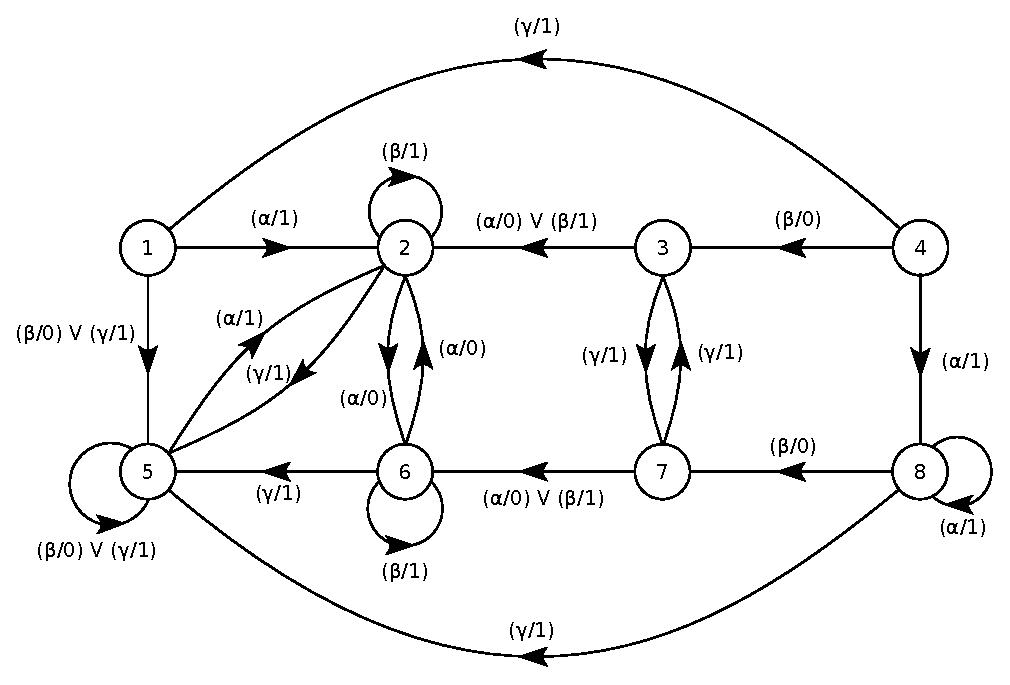
\includegraphics[width=312pt,clip]{images/eps/machineA6}
        \caption{Machine \sampleMachine}
        \label{fig:machineA6}
    \end{figure}


    To illustrate Lemmas \ref{labelSimplyDistinct} to \ref{labelSimplyModifiedEquiv}, consider machine \sampleMachine \label{labelMachineA6}, specified by Fig. \ref{fig:machineA6} and Table \ref{table:transitionA6}. It can be noted that rows 1 and 5 in the transition table are identical and that rows 2 and 6 become identical when every ``2'' is replaced by ``6'' (or every ``6'' is replaced by ``2''). Consequently, each of the state pairs \{1,5\} and \{2,6\} is equivalent. A glance at the $z_\nu$ subtable of \ref{labelMachineA6} reveals that no state in the set \{1,4,5,8\} can be equivalent to any state in the set \{2,3,6,7\}.

    \begin{table}
        \caption{Machine \sampleMachine}
        \label{table:transitionA6}
        \hfill\\
        \centering
        \begin{tabular}{ c || c | c | c || c | c | c }
            \hline
            & \multicolumn{3}{ |c|| }{ $z_\nu $ } & \multicolumn{3}{ |c }{ $s_{\nu+1}$ } \\
            \hline
            \backslashbox{$s_\nu$}{$x_\nu$} & $\alpha$ & $\beta$ & $\gamma$ & $\alpha$ & $\beta$ & $\gamma$ \\
            \hline
            1 & 1 & 0 & 1 & 2 & 5 & 5 \\
            2 & 0 & 1 & 1 & 6 & 2 & 5 \\
            3 & 0 & 1 & 1 & 2 & 2 & 7 \\
            4 & 1 & 0 & 1 & 8 & 3 & 1 \\
            5 & 1 & 0 & 1 & 2 & 5 & 5 \\
            6 & 0 & 1 & 1 & 2 & 6 & 5 \\
            7 & 0 & 1 & 1 & 6 & 6 & 3 \\
            8 & 1 & 0 & 1 & 8 & 7 & 5 \\
            \hline
        \end{tabular}
    \end{table}

\section{\emph{k}-equivalence}

    A notion which will be found useful in further discussions is that of ``\emph{k}-equivalence'':

    \definition \label{labelDefEquivK} State $\sigma_i$ of machine $M_1$ and state $\sigma_j$ of machine $M_2$ are said to be \emph{k}-equivalent, if $M_1|\sigma_i$ and $M_2|\sigma_j$, when excited by an input sequence of length \emph{k}, yield identical output sequences. If $\sigma_i$ and $\sigma_j$ are not \emph{k}-equivalent, they are said to be \emph{k}-distinguishable. $M_1$ and $M_2$ may refer to the same machine.

    Thus, $\sigma_i$ and $\sigma_j$ are \emph{k}-equivalent if and only if there is no way of distinguishing, by using input sequences of length \emph{k} and by observing the external terminals, between machine $M_1$ at state $\sigma_i$ and machine $M_2$ at state $\sigma_j$. $\sigma_i$ and $\sigma_j$ are \emph{k}-distinguishable if and only if there is at least one input sequence of length \emph{k} which, when applied to both $M_1|\sigma_i$ and $M_2|\sigma_j$, yields different output sequences. Two states which are 1-distinguishable are seen to be simply distinguishable, as defined in Sec. \ref{sectionStateEquivalence}.

    From definition \ref{labelDefEquivK} it can be readily verified that \emph{k}-equivalence obeys the reflexive, symmetric, and transitive laws. Consequently, \emph{k}-equivalence can be treated as ordinary equivalence relation and applied directly to sets of states of any size. \emph{k}-distinguishability, on the other hand, does not obey the reflexive and transitive laws, and hence can be applied only to pairs of states.

    \lemma \label{labelDefEquivLemma} \begin{inparaenum}[a)]
        \item If two states are \emph{k}-equivalent, then they are \emph{l}-equivalent for every $ l \leq k $.
        \item If two states are \emph{k}-distinguishable, then they are \emph{l}-distinguishable for every $ l \geq k $
    \end{inparaenum}

    \emph{Proof}. \begin{inparaenum}[a)] 
        \item Suppose $ \sigma_i $ and $ \sigma_j $ are \emph{k}-equivalent but distinguishable by some input sequence, say $ \upvarepsilon_l $, of length $ l \leq k $. Then $ \sigma_i $ and $ \sigma_j $ must be distinguishable by the input sequence $ \upvarepsilon_l \upvarepsilon_{k-l} $ where $ \upvarepsilon_{k-l} $ is any input sequence of length $k - l$. Hence, $ \sigma_i $ and $ \sigma_j $ are \emph{k}-distinguishable, which is a contradiction. 
        \item Suppose $ \sigma_i $ and $ \sigma_j $ are \emph{k}-distinguishable but l-equivalent for some $ l \geq k $. By part \emph{a}, however, if $ \sigma_i $ and $ \sigma_j $ are \emph{l}-equivalent, they must be \emph{k}-equivalent for every $ k \leq l$. By contradiction, then, part \emph{b}, follows.
    \end{inparaenum}

    The state into which state $ \sigma_i $ passes when input sequence of length \emph{k} is applied is called the \emph{kth successor} of $ \sigma_i $ with respect to this sequence. The zeroth successor of a state is the state itself.

    \theorem If states $ \sigma_i $ and $ \sigma_j $ are \emph{k}-equivalent, and if their \emph{k}th successors with respect to any input sequence of length \emph{k} are equivalent, then $\sigma_i = \sigma_j$.

    \emph{Proof}. If $\sigma_i$ and $\sigma_j$ are \emph{k}-equivalent, then, by Lemma \ref{labelDefEquivLemma}, they yield identical responses to all input sequences of length \emph{k} or less. If their \emph{k}th successors, with respect to any input sequence of length \emph{k}, are equivalent, then they yield identical responses to all input sequences which follow the first \emph{k} symbols. Hence, $ \sigma_i $ and $ \sigma_j $ yield identical responses to input sequences of \emph{any} length, which implies that $\sigma_i = \sigma_j$

    \theorem \label{labelBelowKEquiv} If states $ \sigma_i $ and $ \sigma_j $ are equivalent, then their \emph{k}th successor, with respect to any input sequence of length \emph{k} and for any \emph{k}, are equivalent.

    \emph{Proof} Let $ \sigma^{'}_i$ and  $ \sigma^{'}_j$ denote the \emph{k}th successors of $\sigma_i$ and $\sigma_j$, respectively, with respect to an arbitrary input sequence $\upvarepsilon_k$. If $ \sigma^{'}_i \neq \sigma^{'}_j $, then there is a sequence, say $\upvarepsilon_l$, for which $ \sigma^{'}_i $ and $ \sigma^{'}_j $ yield different responses. Hence, the responses of $\sigma_i$ and $\sigma_j$ to $\upvarepsilon_k\upvarepsilon_l$ must be different, which contradicts the assumption that $ \sigma_i = \sigma_j $.

    \begin{figure}[!h]
        \centering
        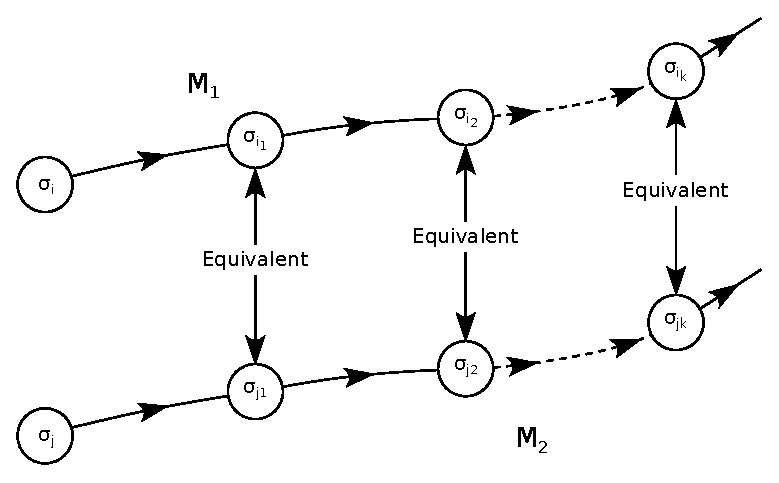
\includegraphics[width=256pt,clip]{images/eps/pathsThroughM1AndM2}
        \caption{Paths traversed in $M_1$ and $M_2$ when $\sigma_i = \sigma_j$ }
        \label{fig:kEquivalenceTraversal}
    \end{figure}

    An input sequence applied to both $M_1|\sigma_i$ and $M_2|\sigma_j$ may be associated with a pair of paths originating in states $\sigma_i$ and $\sigma_j$ in the transition diagram of $M_1$ and $M_2$ respectively. Theorem \ref{labelBelowKEquiv} implies that if the pair of initial states in these paths is equivalent, then every pair of corresponding states in the paths (i.e., states reached from the initial states after the traversal of the same number of branches) is also equivalent. This situation is illustrated in Fig. \ref{fig:kEquivalenceTraversal}, where the shown paths are the paths traversed in $M_1$ and $M_2$ when a certain input sequence is applied to $M_1|\sigma_i$ and $M_2|\sigma_j$. If $\sigma_i$ and $\sigma_j$ are equivalent, then the \emph{k}th successors $\sigma_{i_{k}}$ and $\sigma_{j_{k}}$ must be equivalent for all \emph{k}.

    The preceding results can be used, in many cases, to establish equivalence of states when the equivalence of other states is already established. Suppose, for example, that the pairs of states \{1,5\} and \{3,7\} in machine \ref{labelMachineA6} of Fig. \ref{fig:machineA6} are known to be equivalent. Consequently, the pair \{4,8\} must be equivalent, since 4 and 8 are 1-equivalent, with the pairs \{1,5\} and \{3,7\} being their first successors. If the pair \{4,8\} is known to be equivalent, then the pairs \{1,5\}, \{2,6\} and \{3,7\} must also be equivalent, since they constitute pairs of corresponding states in paths originating in states 4 and 8.

\section{\emph{k}-equivalence Partitions}
\label{labelSectionEquivalenceK}

    For purposes which will become apparent in latter sections, it is of interest to divide, or ``partition'', the states of a machine into classes according to the following criteria: \begin{inparaenum}
    \item All states which belong to the same class must be \emph{k}-equivalent.
    \item All states which belong to different classes must be \emph{k}-distinguishable.
    \end{inparaenum} This partition is called the \emph{k-equivalence partition} of the machine and is denoted by $P_k$. The classes of $P_k$ are called \emph{k-equivalence classes} and are denoted by $\Sigma_{k1},\Sigma_{k2},\Sigma_{k3}$, etc. States belonging to the same class are called \emph{adjoint states}; states belonging to different classes are called \emph{disjoint states}.

    \incSampleMachine
    \begin{figure}[!h]
        \centering
        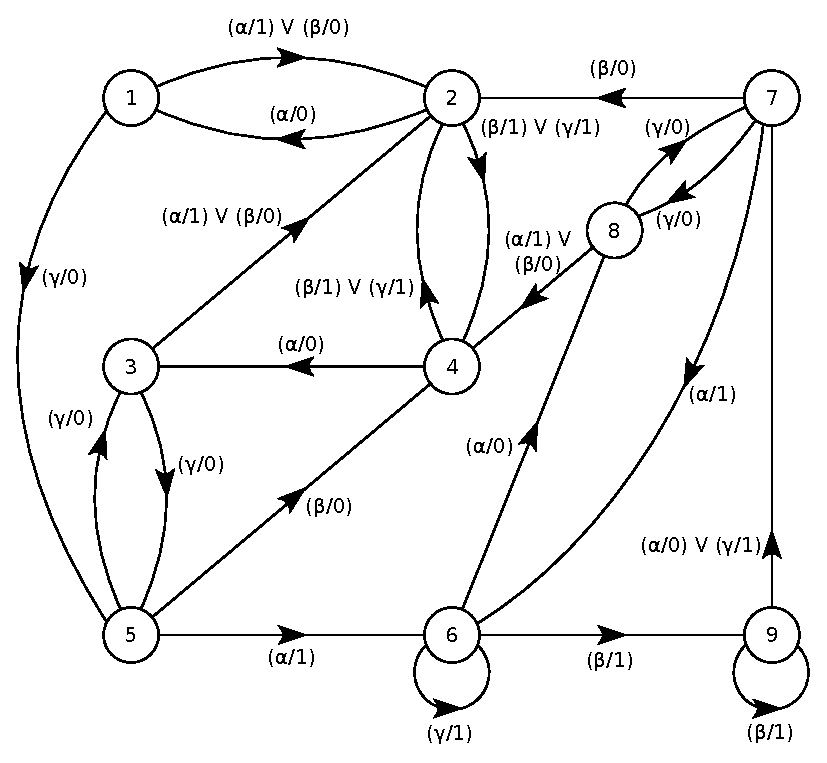
\includegraphics[width=312pt,clip]{images/eps/machineA7}
        \caption{Machine \sampleMachine}
        \label{fig:machineA7}
    \end{figure}

    Figure \ref{fig:machineA7} and Table \ref{table:transitionA7} represent machine \sampleMachine \label{labelMachineA7}. For this machine, the 2-equivalence partition table is given by:

    \begin{align} \label{labelEq2A7}
        {P_2:} \quad{} &\Sigma_{21} = \{1,3,5,7,8\} \nonumber \\
        &\Sigma_{22} = \{2,4,6\} \nonumber \\
        &\Sigma_{23} = \{9\}
    \end{align}

    As can be readily verified through the transition diagram of \ref{labelMachineA7}, adjoint states in $P_2$, as given by (\ref{labelEq2A7}), are 2-equivalent, and disjoint states are 2-distinguishable. No state in \ref{labelMachineA7} is 2-equivalent to state 9 (except state 9 itself), and hence 9 constitutes a single-state class, or a \emph{singleton}.

    Clearly, no state can belong to two different \emph{k}-equivalence classes simultaneously, since this would imply that the state is \emph{k}-distinguishable with respect to itself. Hence, the total number of states in $P_k$ equals the total number of states in the machine.

    \begin{table}[!h]
        \caption{Machine \sampleMachine}
        \label{table:transitionA7}
        \hfill\\
        \centering
        \begin{tabular}{ c || c | c | c || c | c | c }
            \hline
            & \multicolumn{3}{ |c|| }{ $z_\nu $ } & \multicolumn{3}{ |c }{ $s_{\nu+1}$ } \\
            \hline
            \backslashbox{$s_\nu$}{$x_\nu$} & $\alpha$ & $\beta$ & $\gamma$ & $\alpha$ & $\beta$ & $\gamma$ \\
            \hline
            1 & 1 & 0 & 0 & 2 & 2 & 5 \\
            2 & 0 & 1 & 1 & 1 & 4 & 4 \\
            3 & 1 & 0 & 0 & 2 & 2 & 5 \\
            4 & 0 & 1 & 1 & 3 & 2 & 2 \\
            5 & 1 & 0 & 0 & 6 & 4 & 3 \\
            6 & 0 & 1 & 1 & 8 & 9 & 6 \\
            7 & 1 & 0 & 0 & 6 & 2 & 8 \\
            8 & 1 & 0 & 0 & 4 & 4 & 7 \\
            9 & 0 & 1 & 1 & 7 & 9 & 7 \\
            \hline
        \end{tabular}
    \end{table}

    \lemma The \emph{k}-equivalence partition of a machine is unique.
    \emph{Proof}. Suppose $P_k$, consisting of $\Sigma_{k1}, \Sigma_{k2}, ..., \Sigma_{ku}$, is not unique. Then there must be another \emph{k}-equivalence partition, say $ P^{'}_k$, consisting of $\Sigma^{'}_{k1}, \Sigma^{'}_{k2}, ..., \Sigma^{'}_{kv}$ for the same machine. Let $\Sigma_{kr} = \{\sigma_{r1}, \sigma_{r2}, ..., \sigma_{rd}  \}  $. Since the states of $\Sigma_{kr}$ are \emph{k}-equivalent, and since there is no state outside $\Sigma_{kr}$ which is equivalent to any state in $\Sigma_{kr}$, there must be a class in $P^{'}_k$, say $\Sigma^{'}_{ks}$ which consists of the states $\sigma_{r1}, \sigma_{r2}, ..., \sigma_{rd}$ and no other states. Applying this argument to $ r = 1,2,...,u $, it follows that to every class in $P_k$ there corresponds an identical class in $ P^{'}_k$. Since the total number of states in $P^{'}_k$ must be the same as that in $P_k$, $P_k$ and $P^{'}_k$ must be identical, and hence $P_k$ is unique.

    \lemma \label{labelkPlusOneDistinct} States which are disjoint in $P_k$ must also be disjoint in $P_{k+1}$.

    \emph{Proof}. From Lemma \ref{labelDefEquivLemma}, if two states are \emph{k}-distinguishable, they must also be $(\emph{k} + 1)$-distinguishable. The present lemma, then, follows immediately from the definition of $P_k$ and $P_{k+1}$.

    As an example, $P_3$ of machine \ref{labelMachineA7} cannot contain classes such as \{1,3,6\} or \{2,5,9\}, since these classes, as can be deduced from (\ref{labelEq2A7}) contain states which are disjoint in $P_2$.

    \lemma \label{labelKPlusOneDistinguishable} If machine $M$ contains two distinguishable states which are \emph{k}-equivalent, then it must also contain two states which are \emph{k}-equivalent but $(\emph{k}+1)$-distinguishable.

    \emph{Proof}. Let $\sigma_i$ and $\sigma_j$ be the distinguishable states of $M$ which are \emph{k}-equivalent, and let the input sequence $ \xi_{h_{1}}, \xi_{h_{2}}, ..., \xi_{h_{l}} $ be the shortest input sequence which distinguishes between $ \sigma_i $ and $ \sigma_j $. $ \sigma_i $ and $ \sigma_j $, then, yield distinct output symbols when $ \xi_{h_{l}} $ is applied, but not before. Since $ \sigma_i $  and $ \sigma_j $ are \emph{k}-equivalent, we must have $ l > k $. Let the $(\emph{l-k}-1)$st successors of $\sigma_i$ and $\sigma_j$ with respect to $ \xi_{h_{1}} \xi_{h_{2}} ... \xi_{h_{l-k-1}} $ be $\sigma^{'}_i$ and $\sigma^{'}_j$, respectively; since $ l > k, l-k-1 \geq 0 $ and these successors always exist. $\sigma^{'}_i$ and $ \sigma^{'}_j$ then, can be distinguished by the input sequence $ \xi_{h_{l-k}}  \xi_{h_{l-k + 1 }  } ... \xi_{h_{l}} $ whose length is $ l - (l-k-1) = k + 1$. They cannot be distinguished by any shorter sequence, since this would contradict the assumption that $ \sigma_i $ and $\sigma_j$ are \emph{k}-equivalent. Hence, $\sigma^{'}_i$ and $\sigma^{'}_j$ are \emph{k}-equivalent but $(\emph{k}+1)$-distinguishable, which proves the theorem. The above situation is illustrated in Fig. \ref{fig:kPlusOneDistinguishable}.

    \begin{figure}[!h]
        \centering
        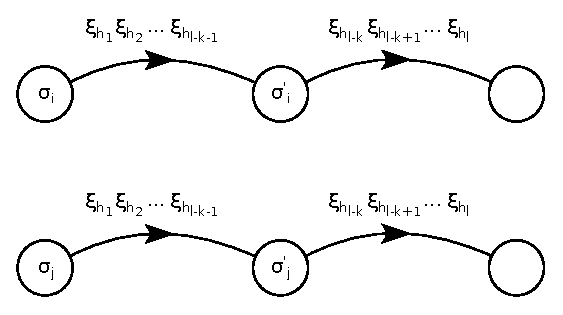
\includegraphics[width=256pt,clip]{images/eps/kPlusOneDistinguishablePath}
        \caption{Illustration for Lemma \ref{labelKPlusOneDistinguishable} }
        \label{fig:kPlusOneDistinguishable}
    \end{figure}

    Suppose now that the adjoint states in each equivalence class of $P_k$ are equivalent. Then, clearly, $P_{k+u}$ is identical with $P_k$ for all nonnegative integers \emph{u}. If two adjoint states in $P_k$ are distinguishable, then they constitute two distinguishable states which are \emph{k}-equivalent. In this case, by Lemma \ref{labelKPlusOneDistinguishable} , the machine must contain two states which are \emph{k}-equivalent but $(\emph{k}+1)$-distinguishable. Hence, $P_k$ must contain two adjoint states which become disjoint in $P_{k+1}$. Thus, if the adjoint states in any class of $P_k$ are distinguishable, $P_{k+1}$ must differ from $P_{k}$. By Lemma \ref{labelkPlusOneDistinct}, if $P_{k+1}$ differs from $P_k$, it must be a ``proper refinement'' of $P_k$, that is, it must be obtainable by splitting one or more classes of $P_k$ into two or more subclasses. In conclusion, the following can be stated:

    \theorem \label{labelRefinement} $P_{k+1}$ must be a proper refinement of $P_k$, unless the adjoing states in every class of $P_k$ are equivalent, in which case $P_k$ and $P_{k+1}$ are identical.

    For machine \ref{labelMachineA7}, for example, we have
    \begin{align} \label{labelEq3A7}
        {P_3:} \quad{} &\Sigma_{31} = \{1,3,5,7,8\} \nonumber \\
        &\Sigma_{32} = \{2,4\} \\
        &\Sigma_{33} = \{6\} \nonumber \\
        &\Sigma_{34} = \{9\} \nonumber
    \end{align}
    which is a proper refinement of $P_2$, and
    \begin{align} \label{labelEq4A7}
        {P_4:} \quad{} &\Sigma_{41} = \{1,3,8\} \nonumber \\
        &\Sigma_{42} = \{2,4\} \nonumber \\
        &\Sigma_{43} = \{5,7\} \\
        &\Sigma_{44} = \{6\} \nonumber \\
        &\Sigma_{45} = \{9\} \nonumber
    \end{align}
    which is a proper refinement of $P_3$, However,
    \begin{align} \label{labelEq5A7}
        {P_5:} \quad{} &\Sigma_{51} = \{1,3,8\} \nonumber \\
        &\Sigma_{52} = \{2,4\} \nonumber \\
        &\Sigma_{53} = \{5,7\} \\
        &\Sigma_{54} = \{6\} \nonumber \\
        &\Sigma_{55} = \{9\} \nonumber
    \end{align}
    is seen to be identical do $P_4$, and hence the adjoint states in every class of $P_4$ are equivalent.

\section{Equivalence Partitions}
\label{labelSectionEquivPartitions}

A \emph{k}-equivalence partition for machine $M$ is called an \emph{equivalence partition} of $M$, and denoted by $ \widehat{P} $, if the adjoint states in every class of this partition are equivalent. Under these conditions, each class in the partition is called an \emph{equivalence class}. From the discussion in \ref{labelSectionEquivalenceK} it follows that $ \widehat{P} $ is the most refined $P_k$ partition. By Theorem \ref{labelRefinement}, $ \widehat{P} $ can be obtained by constructing $P_k$ for $ \emph{k} = 1,2,3...$, until, for the first time, a partition is produced which is identical to the one previously produced; this partition is $ \widehat{P} $. Let $P_i = P_j $ signify the fact that $P_i$ and $P_j$ are identical partitions, and let $|P_i|$ denote the number of classes in $P_i$. Using this notation, the preceding results can be summarized as follows:

\begin{equation} \label{labelEqRefinement}
    |P_k| \leq |P_{k+1} |
\end{equation}
    If $|P_k| = |P_{k+1}|$, then
\begin{equation} \label{labelEqMostRefined}
    P_k = P_{k+u} = \widehat{P} \qquad{} u = 0, 1, 2, ...
\end{equation}

% TODO: adicionar defini��o introduzida na se��o 1.6 e alterar referencia no paragrafo abaixo

If all the states in a given \emph{n}-state machine are 1-equivalent, $P_1$ consists of a single class containing \emph{n} states. Clearly, if all \emph{n} states are 1-equivalent, their first successors, with respect to any input sequence, are also 1-equivalent. Consequently, all \emph{n} states must be 2-equivalent, and hence $P_1 = P_2$. By (\ref{labelEqMostRefined}), then, $P_1 = \widehat{P}$, and all \emph{n} states are equivalent. For a machine of this type, $f_{z}(x_{\nu}, s_{\nu})$ is the same for all $s_{\nu}$, and hence $f_{z}(x_{\nu}, s_{\nu}) = f_{z}( x_{\nu} )$. From the definition introduced in section 1.6, then, it can be stated that a machine in which all states are equivalent is a trivial machine. Unless otherwise specified, further discussion will be confined to nontrivial machines only, i.e., to machines in which there is at least one distinguishable pair of states, or in whose 1-equivalence partition there are at least two classes.

    \lemma \label{labelNeqPartitions} If $P_k \neq P_{k-1}$ then
    \begin{equation} \label{labelEqProperRefinement}
        |P_k| \geq k + 1
    \end{equation}

    \emph{Proof}. If $P_k \neq P_{k-1} $, then, by (\ref{labelEqRefinement}) and (\ref{labelEqMostRefined}), $ |P_r| > |P_{r-1}| $ for $ \emph{r} = 1,2,...,\emph{k} $. Since $ P_1 \geq 2 $, (\ref{labelEqProperRefinement}) follows by induction.

    \lemma If for an \emph{n}-state machine $ P_k \neq P_{k-1} $, then the number of states in each class of $P_k$ is at most $ n - k $.

    \emph{Proof}. By Lemma \ref{labelNeqPartitions}, the number of classes in $P_k$ is at least $k+1$. Suppose one class contains more than $n-k$, say $n-k+1$ states. Then, since every other class in $P_k$ must contain at least one state, the total number of states in $P_k$ is at least $ k + (n-k+1) = n+1 $. Since the total number of states cannot exceed \emph{n}, the lemma follows by contradiction.

    \lemma \label{labelLastMostRefined} In an \emph{n}-state machine, $P_n = P_{n-1}$.

    \emph{Proof}. If $P_n \neq P_{n-1}$, then, by Lemma \ref{labelNeqPartitions}, $|P_n| \geq n+1 $. Since the number of classes in a \emph{k}-equivalence partition of an \emph{n}-state machine cannot exceed \emph{n}, the lemma follows by contradiction.

    From Lemma \ref{labelLastMostRefined} and \ref{labelEqMostRefined}, the following can be concluded:

    \theorem \label{labelTheoremLastMostRefined} In an \emph{n}-state machine,
    \begin{equation}
        P_{n-1} = \widehat{P}
    \end{equation}

    Thus, in the process of determining $\widehat{P}$ for an \emph{n}-state machine, by successively constructing $P_k$ for $ \emph{k} = 1, 2, 3, ...$, at most $n-1$ such constructions are needed. An alternative formulation of Theorem \ref{labelTheoremLastMostRefined} is the following:

    \corollary Two states in an \emph{n}-state machine are equivalent if they are $(\emph{n}-1)$-equivalent and distinguishable if they are $(\emph{n-1})$-distinguishable.


    \emph{Determination of} $P_1$. $P_1$ can be determined through the following rule: 
    States are adjoint in $P_1$ if and only if, for every input symbol, they yield identical output symbols.


    \emph{Determination of} $P_{k+1}$ \emph{from} $P_k(\emph{k}\geq1)$. A pair of adjoint states in $P_k$ which, for every input symbol, pass into adjoint states in $P_k$ represent \emph{k}-equivalent states whose first successors, with respect to every input symbol, are \emph{k}-equivalent. Such adjoint states, then, are $(\emph{k}+1)$-equivalent and must be adjoint in $P_{k+1}$. A pair of adjoint states in $P_k$ which, for some input symbol, pass into disjoint states in $P_k$ represent \emph{k}-equivalent states whose first successors, with respect to some input symbol, are \emph{k}-distinguishable. Such adjoint states are $(\emph{k}+1)$-distinguishable and must be disjoint in $P_{k+1}$. A pair of disjoint states in $P_k$ must be disjoint in $P_{k+1}$. Thus $P_{k+1}$ can be determined from $ P_k $ by dividing the states of every class in $P_k$ into subclasses, such that two states are in the same subclass if and only if their first successors, with respect to every input symbol, are adjoint states in $P_k$. The resulting subclasses are the classes of $P_{k+1}$. Since singletons cannot be divided into subclasses, singletons which appear in $P_k$ can be automatically assigned as singletons to $P_{k+1}$.

    Consider, for example, $P_3$ of machine \ref{labelMachineA7}, as given in (\ref{labelEq3A7}). The first successors of states 1, 3, and 8 are adjoint in $\Sigma_{32}$ when $\alpha$ or $\beta$ is applied and in $\Sigma_{31}$ when $\gamma$ is applied. The first successors of states 5 and 7 are adjoint in $\Sigma_{33}$ when $\alpha$ is applied, in $\Sigma_{32}$ when $\beta$ is applied, and in $\Sigma_{31}$ when $\gamma$ is applied. Consequently, \{1,3,8\} and \{5,7\} are classes of $P_4$. The first successors of states 2 and 4, with respect to every input symbol, are adjoint states in $P_3$; \{2,4\}, therefore, is a class in $P_4$. The singletons \{6\} and \{9\} appear as singletons in $P_4$. The resulting partition $P_4$, then, is as shown in (\ref{labelEq4A7}).

    We have thus outlined the criteria for the successive construction of $P_k$, for $\emph{k} = 1,2,3,...$. When, for every input symbol, every pair of adjoint states in $P_k$ passes into adjoint states in $P_k$, no further refinement of $P_k$ is possible, and hence $P_k = \widehat{P}$. The outlined criteria, then, lead to the determination of the equivalence partition of the given machine.

\section{Partitioning by \emph{$P_k$} Tables}
\label{section:partitionByPkTables}

    In any but the simplest cases, the process of determining the equivalence partition of a given machine by inspection of the transition table, diagram, or matrix is virtually impossible. In this section we shall describe a method by which the partitioning can be carried out sistematically, by constructing a series of so-called $P_k$ tables.

\begin{table}[h]
\parbox{ .45\linewidth }{
    \begin{tabular}{ c c | c | c  | c }
        \cline{3-5} &  & \multicolumn{3}{ c  }{ $s_{\nu+1}$ } \\
        \hline 
        \multicolumn{1}{c|}{ $ \Sigma $ } & \backslashbox{$s_\nu$}{ $x_{\nu}$  } & $\alpha$ & $\beta$ & $\gamma$ \\
        \hline
        \multicolumn{1}{c|}{ \multirow{5}{*}{a}}  & 1 & $2_b$ & $2_b$ & $5_a$  \\
        \multicolumn{1}{c|}{} & 3 & $2_b$ & $2_b$ & $5_a$ \\
        \multicolumn{1}{c|}{} & 5 & $6_b$ & $4_b$ & $3_a$ \\
        \multicolumn{1}{c|}{} & 7 & $6_b$ & $2_b$ & $8_a$ \\
        \multicolumn{1}{c|}{} & 8 & $4_b$ & $4_b$ & $7_a$ \\
        \hline
        \multicolumn{1}{c|}{ \multirow{4}{*}{b}}  & 2 & $1_a$ & $4_b$ & $4_b$ \\
        \multicolumn{1}{c|}{} & 4 & $3_a$ & $2_b$ & $2_b$ \\
        \multicolumn{1}{c|}{} & 6 & $8_a$ & $9_b$ & $6_b$ \\
        \multicolumn{1}{c|}{} & 9 & $7_a$ & $9_b$ & $7_a$ \\
        \hline
    \end{tabular}
    \caption{ $P_1$ Table for \ref{labelMachineA7} }
    \label{table:tableP1A7}
}
\qquad{}
\parbox{ .45\linewidth }{
    \begin{tabular}{ c c | c | c  | c }
        \cline{3-5} &  & \multicolumn{3}{ c  }{ $s_{\nu+1}$ } \\
        \hline 
        \multicolumn{1}{c|}{ $ \Sigma $ } & \backslashbox{$s_\nu$}{ $x_{\nu}$  } & $\alpha$ & $\beta$ & $\gamma$ \\
        \hline
        \multicolumn{1}{c|}{ \multirow{5}{*}{a}}  & 1 & $2_b$ & $2_b$ & $5_a$  \\
        \multicolumn{1}{c|}{} & 3 & $2_b$ & $2_b$ & $5_a$ \\
        \multicolumn{1}{c|}{} & 5 & $6_b$ & $4_b$ & $3_a$ \\
        \multicolumn{1}{c|}{} & 7 & $6_b$ & $2_b$ & $8_a$ \\
        \multicolumn{1}{c|}{} & 8 & $4_b$ & $4_b$ & $7_a$ \\
        \hline
        \multicolumn{1}{c|}{ \multirow{3}{*}{b}}  & 2 & $1_a$ & $4_b$ & $4_b$ \\
        \multicolumn{1}{c|}{} & 4 & $3_a$ & $2_b$ & $2_b$ \\
        \multicolumn{1}{c|}{} & 6 & $8_a$ & $9_c$ & $6_b$ \\
        \hline
        \multicolumn{1}{c|}{c} & 9 & $7_a$ & $9_c$ & $7_a$ \\
        \hline
    \end{tabular}
    \caption{ $P_2$ Table for \ref{labelMachineA7} }
    \label{table:tableP2A7}
}
\end{table}

The $P_k$ table of a given machine is essentially the same as the $ s_{\nu+1} $ subtable for that machine, with the following modifications: \begin{inparaenum}[ (1)] 
\item If $\{ \sigma_{i_{1}}, \sigma_{i_{2}}, ..., \sigma_{i_{r}} \}$ is a class in $ P_k $, rows $ \sigma_{i_{1}}, \sigma_{i_{2}}, ..., \sigma_{i_{r}} $ are grouped together, each group separated from the adjacent ones by a rule. The order of the groups in the table and the order of the rows within each group are arbitrary. Rows which belong to the same group, and hence represents a \emph{k}-equivalence class, will be called \emph{adjoint rows}; rows which belongs to different groups will be called \emph{disjoint rows}.
    \item A ``$\Sigma$'' column is added, which labels each group of rows in the $P_k$ table. The labels are arbitrary and may be chosen independently in each new $P_k$ table.
    \item A subscript is attached to every $s_{\nu+1}$ entry, which identifies the group in the $P_k$ table to which the entry belongs. Thus, if row $\sigma_i$ is in the group labeled ``a'', then every $s_{\nu+1}$ entry ``$\sigma_i$'' is assigned the subscript ``a''.
    \end{inparaenum}

    Tables \ref{table:tableP1A7} to \ref{table:tableP4A7} are the $P_1, P_2, P_3$, and $P_4$ tables for machine \ref{labelMachineA7} of Figure \ref{fig:machineA7}.

    \emph{Construction of the $P_1$ Table}. Reorder the rows of the transition table so that rows which are identical in the $z_\nu$ subtable become adjacent. Each group of such rows corresponds to a 1-equivalence class, and hence to a group of adjoint rows in the $P_1$ table. The $P_1$ table can now be constructed by deleting the $z_{\nu}$ subtable, separating the row groups by rules, adding a ``$\Sigma$'' column, and subscripting the $s_{\nu} + 1$ entries as described above. For an illustration, refer to Tables \ref{table:transitionA7} and \ref{table:tableP1A7}.

\begin{table}[h]
\parbox{ .45\linewidth }{
    \begin{tabular}{ c c | c | c  | c }
        \cline{3-5} &  & \multicolumn{3}{ c  }{ $s_{\nu+1}$ } \\
        \hline 
        \multicolumn{1}{c|}{ $ \Sigma $ } & \backslashbox{$s_\nu$}{ $x_{\nu}$  } & $\alpha$ & $\beta$ & $\gamma$ \\
        \hline
        \multicolumn{1}{c|}{ \multirow{5}{*}{a}}  & 1 & $2_b$ & $2_b$ & $5_a$  \\
        \multicolumn{1}{c|}{} & 3 & $2_b$ & $2_b$ & $5_a$ \\
        \multicolumn{1}{c|}{} & 5 & $6_c$ & $4_b$ & $3_a$ \\
        \multicolumn{1}{c|}{} & 7 & $6_c$ & $2_b$ & $8_a$ \\
        \multicolumn{1}{c|}{} & 8 & $4_b$ & $4_b$ & $7_a$ \\
        \hline
        \multicolumn{1}{c|}{ \multirow{2}{*}{b}}  & 2 & $1_a$ & $4_b$ & $4_b$ \\
        \multicolumn{1}{c|}{} & 4 & $3_a$ & $2_b$ & $2_b$ \\
        \hline
        \multicolumn{1}{c|}{c} & 6 & $8_a$ & $9_d$ & $6_c$ \\
        \hline
        \multicolumn{1}{c|}{d} & 9 & $7_a$ & $9_d$ & $7_a$ \\
        \hline
    \end{tabular}
    \caption{ $P_3$ Table for \ref{labelMachineA7} }
    \label{table:tableP3A7}
}
\qquad
\parbox{ .45\linewidth }{
    \begin{tabular}{ c c | c | c  | c }
        \cline{3-5} &  & \multicolumn{3}{ c  }{ $s_{\nu+1}$ } \\
        \hline 
        \multicolumn{1}{c|}{ $ \Sigma $ } & \backslashbox{$s_\nu$}{ $x_{\nu}$  } & $\alpha$ & $\beta$ & $\gamma$ \\
        \hline
        \multicolumn{1}{c|}{ \multirow{3}{*}{a}}  & 1 & $2_b$ & $2_b$ & $5_c$  \\
        \multicolumn{1}{c|}{} & 3 & $2_b$ & $2_b$ & $5_c$ \\
        \multicolumn{1}{c|}{} & 8 & $4_b$ & $4_b$ & $7_c$ \\
        \hline
        \multicolumn{1}{c|}{ \multirow{2}{*}{b}}  & 2 & $1_a$ & $4_b$ & $4_b$ \\
        \multicolumn{1}{c|}{} & 4 & $3_a$ & $2_b$ & $2_b$ \\
        \hline
        \multicolumn{1}{c|}{ \multirow{2}{*}{c}} & 5 & $6_d$ & $4_b$ & $3_a$ \\
        \multicolumn{1}{c|}{} & 7 & $6_d$ & $2_b$ & $8_a$ \\
        \hline
        \multicolumn{1}{c|}{d} & 6 & $8_a$ & $9_e$ & $6_d$ \\
        \hline
        \multicolumn{1}{c|}{e} & 9 & $7_c$ & $9_e$ & $7_c$ \\
        \hline
    \end{tabular}
    \caption{ $P_4$ Table for \ref{labelMachineA7} }
    \label{table:tableP4A7}
}

\end{table}

\emph{Construction of the $P_{k+1}$ Table from the $P_k$ Table $(k\geq 1)$}. A pair of adjoint rows in the $P_k$ table which, in every column, exhibit identical subscripts are adjoint rows in the $P_{k+1}$ table. A pair of adjoint rows in the $P_k$ table which, in some column, exhibit different subscripts are disjoint rows in the $P_{k+1}$ table. Disjoint rows in the $P_{k}$ table are also disjoint in the $P_{k+1}$ table. A group in the $P_k$ table consisting of a single row remains a single-row group in the $P_{k+1}$ table. Thus, the groups of the $P_{k+1}$ tables can be estabilished by inspection of the subscripts in the $P_k$ table. Once the groups are estabilished, the table itself can be constructed according to the format stipulated above. The justification for the foregoing rules follows directly from the manner in which the subscripts are assigned and from the criteria for determining $P_{k+1}$ from $P_k$, as outlined in Section \ref{labelSectionEquivPartitions}.

    As an example, consider the $P_3$ table for \ref{labelMachineA7}, shown in Table \ref{table:tableP3A7}. In group ``a'', rows 1, 3 and 8 have identical subscripts in every column, and so do rows 5 and 7 (whose subscripts differ from those of 1, 3 and 8).

    Consequently, rows 1, 3 and 8 and rows 5 and 7 constitute two groups of rows in the $P_4$ table. In group ``b'' all rows exhibit identical subscripts in every column, and hence the group remains intact in the $P_4$ table. Groups ``c'' and ``d'', consisting of one row each, can be transferred intact to the $P_4$ table.

    Given a procedure for constructing the $P_1$ table, and the $P_{k+1}$ table from the $P_k$ table $( k \geq 1 )$, one can construct the $P_k$ table for successive values of \emph{k}, until a table is obtained in which all adjoint rows exhibit identical subscripts in every column. The stub entries of these adjoint rows represent equivalent states, and hence the group of stub entries in this table represent the desired equivalence classes. By Theorem \ref{labelTheoremLastMostRefined}, this condition must occur for some value of $\emph{k} \leq n - 1$. For machine \ref{labelMachineA7} the condition is exhibited by the $P_4$ table in Table \ref{table:tableP4A7}. The equivalence partition of \ref{labelMachineA7} is, therefore, given by

\begin{equation}
    P: \quad{} \{1,3,8\}, \{2,4\}, \{5,7\}, \{6\}, \{9\} 
\end{equation}
